\documentclass{article}

\usepackage{graphicx}
\usepackage{tikz}
\usepackage{tikzsymbols}
\usetikzlibrary{calc,patterns,shapes.geometric}
\pagestyle{empty}
\usepackage[margin=0pt]{geometry}
\geometry{papersize={14in,12in}}

\def\centerarc[#1](#2)(#3:#4:#5){\draw[#1] ($(#2)+({#5*cos(#3)},{#5*sin(#3)})$) arc (#3:#4:#5);}

\begin{document}
	\begin{figure}
		\centering
		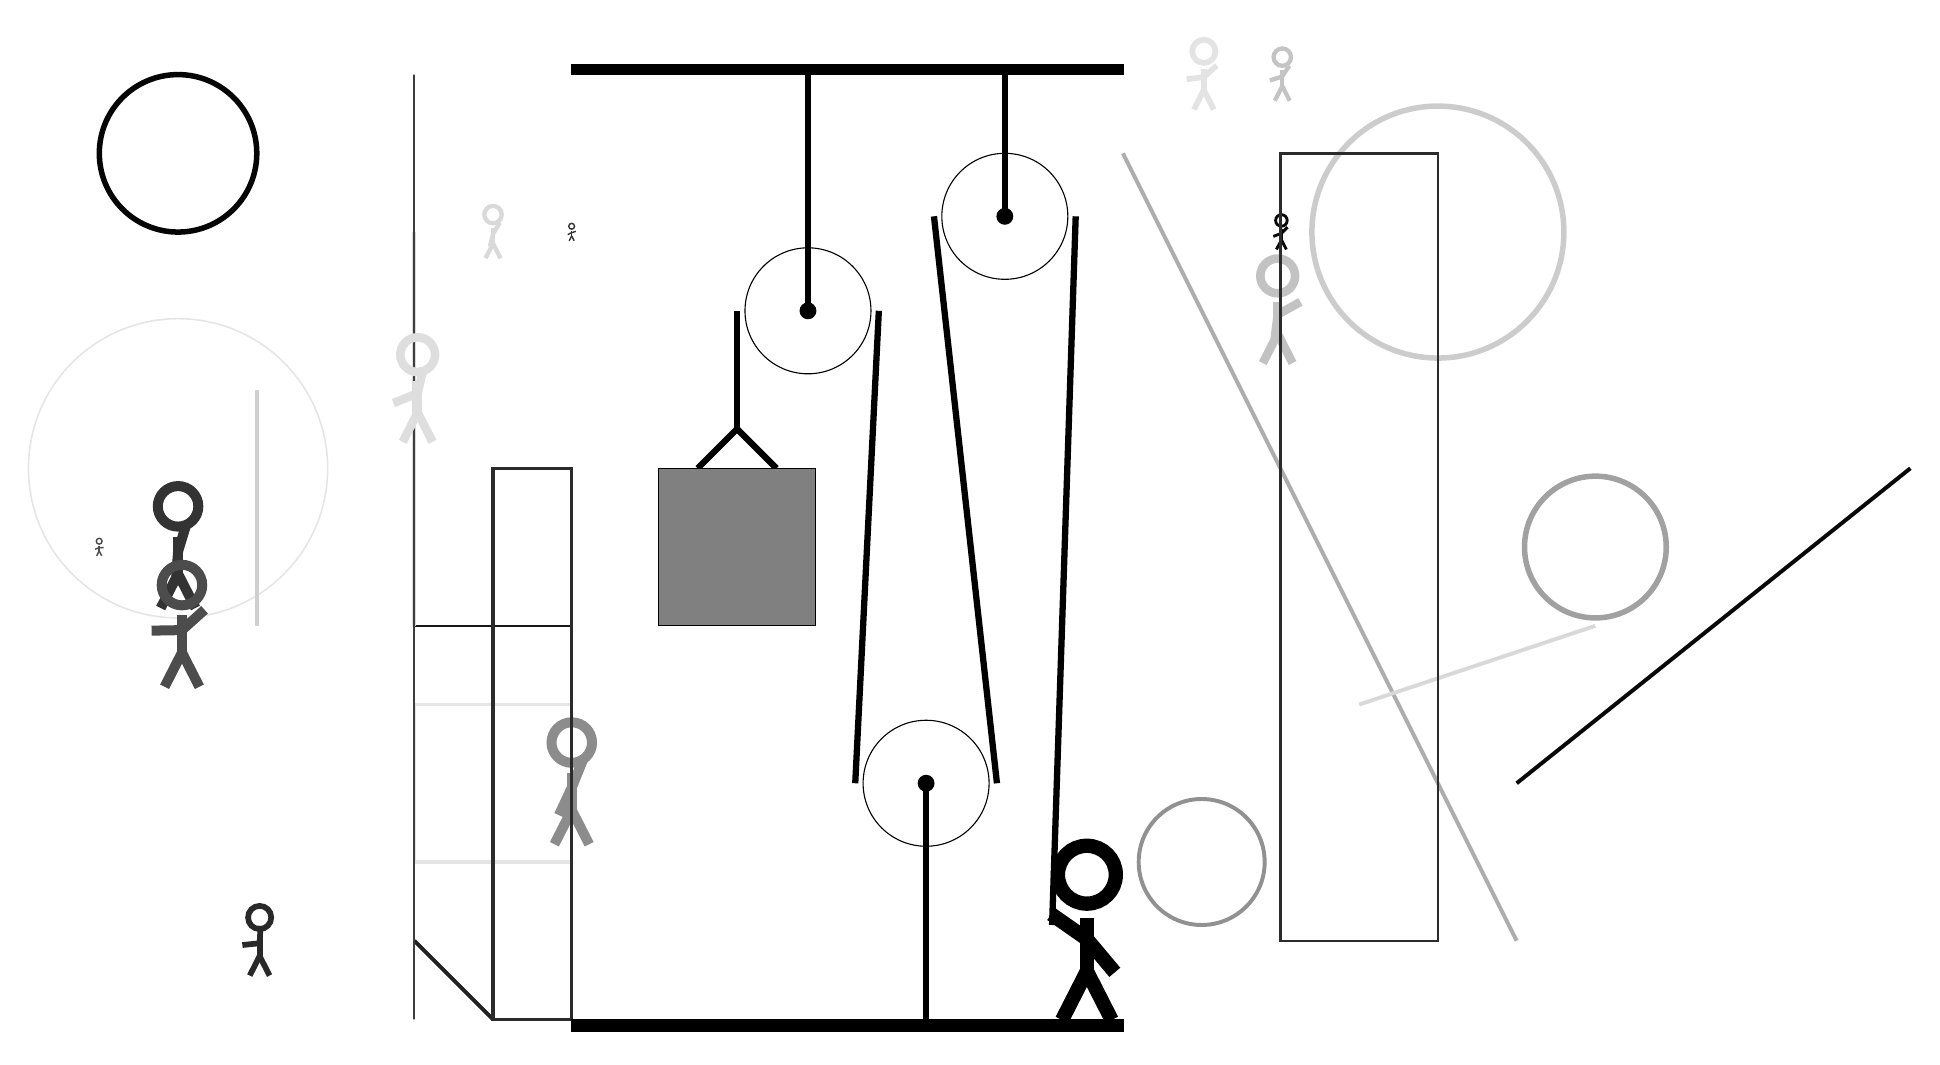
\begin{tikzpicture}
			%%%%% START %%%%%
			
			\draw[fill=black] (-2, 9) rectangle (5, 9.125);
			
			\draw (1, 6) circle (0.8);
			\draw[fill=black] (1, 6) circle (0.1);
			\draw[line width=0.8mm]  (1, 9) -- (1, 6);
			
			\draw[fill=white](2.5, 0) circle (0.8);
			\draw[fill=black] (2.5, 0) circle (0.1);
			\draw[line width=0.8mm]  (2.5, -3) -- (2.5, 0);
			
			\draw[fill=white](3.5, 7.2) circle (0.8);
			\draw[fill=black] (3.5, 7.2) circle (0.1);
			\draw[line width=0.8mm] (3.5, 9) -- (3.5, 7.2);
			
			\draw [line width=0.7mm, color=black!20](9, 7) circle (1.6);
			
			\draw[line width=0.3mm, color=black!90] (-4, 2) rectangle (-2, 2);
			\node[line width=0.2mm, color=black!45] at (-2, 0) {\Strichmaxerl[7][65][68]};
			\draw [line width=0.5mm, color=black!43](6, -1) circle (0.8);
			
			\node[line width=0.5mm, color=black!23] at (7, 9) {\Strichmaxerl[3][18][57]};
			
			\draw [line width=0.7mm, color=black!98](-7, 8) circle (1.0);
			\node[line width=0.2mm, color=black!80] at (-2, 7) {\Strichmaxerl[1][26][18]};
			\draw [line width=0.2mm, color=black!10](-7, 4) circle (1.9);
			\draw [line width=0.7mm, color=black!37](11, 3) circle (0.9);
			
			\node[line width=0.6mm, color=black!84] at (-6, -2) {\Strichmaxerl[4][6][87]};
			\draw[line width=0.5mm, color=black!87](-3, -3) -- (-4, -2);
			\draw[line width=0.4mm, color=black!10] (-4, -1) rectangle (-2, 1);
			\draw[line width=0.5mm, color=black!32](10, -2) -- (5, 8);
			
			\draw[line width=0.5mm, color=black!97](10, 0) -- (15, 4);
			\node[line width=0.4mm, color=black!24] at (7, 6) {\Strichmaxerl[6][83][29]};
			\node[line width=0.6mm, color=black!97] at (7, 7) {\Strichmaxerl[2][21][45]};
			
			\node[line width=0.6mm, color=black!80] at (-7, 3) {\Strichmaxerl[7][86][73]};
			\draw[line width=0.5mm, color=black!15](8, 1) -- (11, 2);
			\draw[line width=0.5mm, color=black!14] (-4, 2) rectangle (-4, 7);
			\node[line width=0.4mm, color=black!11] at (6, 9) {\Strichmaxerl[4][7][42]};
			\draw[line width=0.4mm, color=black!83] (-2, 4) rectangle (-3, -3);
			
			\node[line width=0.4mm, color=black!70] at (-8, 3) {\Strichmaxerl[1][21][1]};
			\draw[line width=0.3mm, color=black!76] (-4, 9) rectangle (-4, -3);
			\node[line width=0.2mm, color=black!13] at (-4, 5) {\Strichmaxerl[6][22][77]};
			\draw[line width=0.5mm, color=black!19](-6, 2) -- (-6, 5);
			\node[line width=0.4mm, color=black!70] at (-7, 2) {\Strichmaxerl[7][1][42]};
			\draw[line width=0.3mm, color=black!83] (7, 8) rectangle (9, -2);
			\node[line width=0.3mm, color=black!15] at (-3, 7) {\Strichmaxerl[3][76][59]};
			
			\draw[line width=0.8mm] (-0.4, 4.0) -- (0.1, 4.5) -- (0.6, 4.0);
			\draw[fill=black!50] (-0.9, 4.0) rectangle (1.1, 2.0);
			
			\draw[line width=0.8mm] (0.1, 6) -- (0.1, 4.5);
			\centerarc[line width=0.8mm](1, 6)(0:180:0.9);
			\draw[line width=0.8mm](1.9, 6) -- (1.6, 0);
			\centerarc[line width=0.8mm](2.5, 0)(180:360:0.9);
			\draw[line width=0.8mm](3.4, 0) -- (2.6, 7.2);
			\centerarc[line width=0.8mm](3.5, 7.2)(0:180:0.9);
			\draw[line width=0.8mm](4.4, 7.2) -- (4.1, -1.8);
			
			\node at (4.5, -1.9) {\Strichmaxerl[10][-35][-50]};
			
			\draw[fill=black] (-2, -3) rectangle (5, -3.15);
			
			%%%%% END %%%%%
		\end{tikzpicture}
	\end{figure}	
\end{document}